\section{GFI}

GFI est une ESN et le stage a eu lieu dans les locaux de la \textbf{Forge}.
\subsection{L'entreprise}

Fondée en 1995, GFI est une Entreprise de Service Numérique (\textit{ESN}) dont le siège se trouve à Saint-Ouen en France. Elle compte aujourd'hui 16 000 collaborateurs dans une vingtaine de pays (Suisse, Belgique, Espagne, Brésil...). Son chiffre d'affaires s'élève à 1 132 M€ en 2017 et 74,5 \% de son activité se situe en France.
\begin{quotation}
\textit{Notre stratégie~: Être reconnu comme le 1er acteur régional des services et solutions à valeur ajoutée.
}
Vincent Rouaix - Président-Directeur Général
\end{quotation}
Pour parvenir à cela GFI a trois leviers de croissances~: 
\begin{itemize}
\item La \textbf{proximité}, avec des implantations régionales qui ont vocation à être souple et réactives pour être à proximité des clients.
\item L'\textbf{industrialisation}, avec à la clef des gains de productivité, une réduction du\textit{ time-to-market} et des coûts optimisés.
\item L'\textbf{innovation} pour apporter des solutions innovantes.
\end{itemize}

Afin de concrétiser le levier de l'innovation, GFI a notamment lancé un \textit{Fablab} dans les locaux du \textbf{Cargo} dans les 19e arrondissement de Paris.

\subsection{La Forge}

\begin{minipage}{0.3\textwidth}
  \centering
  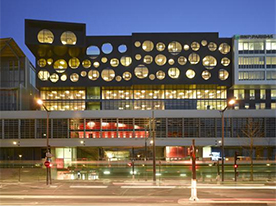
\includegraphics[width=5cm, trim={0 0.5cm 0 0.2cm},clip]{img/cargo.jpg}
\end{minipage}
\hfill%
\begin{minipage}[adjusting]{0.6\textwidth}
 \hspace{\parindent}En octobre 2016, GFI a lancé son Fablab dans les locaux de l'incubateur \textit{Le Cargo} à Paris. Ce Fablab vient renforcer la phase amont du processus d’\textbf{idea generation}. Au travers d’ateliers thématiques, il a vocation de prototyper les cas d’usage des clients.  Pour prolonger cette initiative, GFI a lancé \textit{La Forge}.
\end{minipage}\par

La Forge a pour vocation d'accompagner les entreprises dans l'industrialisation du prototype. Ses experts conseillent les entreprises en matière de financement, de sourcing matériel ou encore de maintenance de l'innovation. En amont, ils ont aussi un rôle de veille technologique et organisent des journées d'acculturation aux «~\textit{buzzwords}~» (machine learning, chatbot...)~: ce que ces nouvelles techniques permettent ou ne permettent pas, en donnant les clefs de compréhensions aux clients pour qu'ils se projettent...

\subsection{Organisation}

La Forge gère plusieurs \textbf{missions en parallèle}, elles peuvent concerner la \textit{Computer Vision}, mais aussi des \textit{chatbots}, des questions de \textit{blockchain}. L'équipe au complet compte près d'une vingtaine de personne qui se répartissent ces différentes missions.

L'équipe est \textbf{composée} d'employés de GFI à plein temps, d'alternants et de stagiaires. 

% AGILE ?


\newpage
